\chapter{Background Research}
\label{CHAP_SECOND}
\centerline{\rule{149mm}{.02in}}
\vspace{2cm}

\section{Overview}
This section will introduce the key concepts and technologies involved with this project, starting from a very high level and moving into specialised areas more relevant to OpenStack. The aim here is to give some context to the work that will be done, provide a foundation for the project and allow  the reader to explore further into relevant source material by following the references I provide.\\ 
Once the initial topics have been introduced, I will bring these together and discuss my plan for OpenStack, including critically assessing some existing papers with the same aim, so as to improve upon them and provide a better solution.

\section{Cloud Computing}
\subsection{Introduction}
Cloud Computing is an area of computing which is very high level, and so difficult to precisely define. It's increase in popularity in recent years have seen it come to the forefront of Computing Technology, and this trend is likely to continue for many years. Many companies now offer 'Cloud Solutions' such as Amazon's Amazon Web Services (AWS) \cite{awsec2} and Microsoft's Windows Azure \cite{winazure}. \\ 
In this part of the research, topics considered include the definition of Cloud Computing, its history and the evolution of the cloud industry. Also covered are the different forms of Cloud Computing services, and some real world applications of Cloud Computing.  

\subsection{Definition}
There are many different definitions of Cloud Computing \cite{21definitions}, each giving some insight to the perspective of the person or organisation coining the definition. The National Institute of Standards and Technology (NIST), for example, defines Cloud Computing as: "\textit{a model for enabling ubiquitous, convenient, on-demand network access to a shared pool of configurable computing resources (e.g., networks, servers, storage, applications, and services) that can be rapidly provisioned and released with minimal management effort or service provider interaction}." \cite{nistcloud} \\
McKinsey \& Co. gave a slightly different definition: “\textit{Clouds are hardware based services offering compute, network, and storage capacity where: Hardware management is highly abstracted from the buyer, buyers incur infrastructure costs as variable OPEN, and infrastructure capacity is highly elastic}” \cite{mickinseyclearingtheair} 
From these definitions, there emerged a number of key common characteristics that define a cloud. Most of these were captured by Armburst et al\cite{armbrustberkeleyview}, and consist of:

\begin{itemize}
\itemsep0em
\item Abstraction - The illusion of infinite resources; Often using Virtualisation. 
\item Pay-per-use - The ability to pay for use as needed;
\item Elimination of start-up commitments by cloud users;
\item Self-service interfaces to reduce necessity of human involvement in process. This is a way of automating cloud management processes. 
\end{itemize} 

The main idea is linked to utility computing, and delivering computing to a consumer as a utility, or as a 'service'\cite{armbrustberkeleyview}. This is a large part of cloud computing will be covered in more detail in other parts of this section. 
Overall, there is no clear definition of Cloud Computing; it appears to be a very high level concept or 'umbrella term' covering on-demand computing services aimed at consumers and businesses.\cite{buyyacloudemerging}.   
 
\subsection{Types of Cloud}
There are a number of different 'types' of cloud, also known as \textbf{Deployment Models}. Each of these has uses and suits a particular situations or needs, and so they successfully co-exist. The three main models, illustrated in the below figure, are public, private and hybrid clouds. 

\begin{figure}[ht]
\centering
\fbox{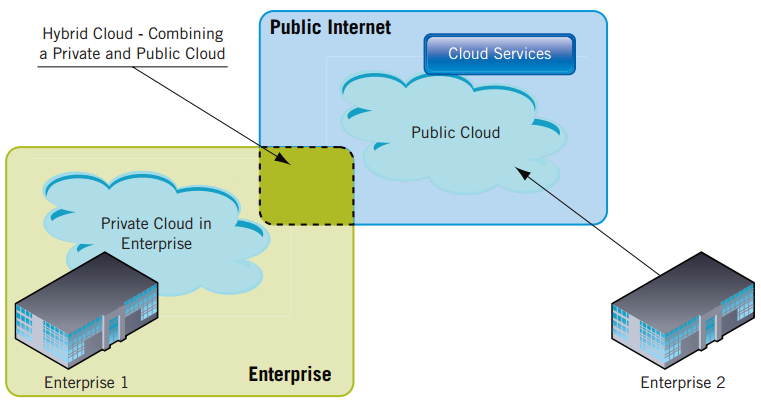
\includegraphics[scale=0.35]{cloud_types}}
\caption[An example figure.]{Cloud Deployment Models \cite{dialogiccloud}.}
\end{figure}

Armbrust et al. \cite{armbrustberkeleyview} define a \textbf{Public Cloud} as a "\textit{cloud made available in a pay-as-you-go manner to the general public}". A Cloud Service Provider (CSP) such as Amazon makes such cloud infrastructures available. This version of a cloud is ideal for start up companies, who may acquire resources without any of the start-up costs associated with developing in-house infrastructure\cite{amazonwhatiscloudcomputing}. Another advantage of a public cloud is the high limit of resources available - using the resources of a global cloud provider gives the potential of enormous elasticity, as they are prepared to service huge demand from a large consumer base. An example of a public cloud service is Google's App Engine, which lets consumers build and run applications on Google's infrastructure, accessed using the internet\cite{googleappengine}. \\ \\
The same publication \cite{armbrustberkeleyview} defines a \textbf{Private Cloud} as "\textit{internal data center of a business or other organisation, not made available to the general public}". Using a private cloud, companies can have more control over their infrastructure, whilst keeping many of the advantages of a cloud, such as the self-service interface. Security of these systems is a huge advantage, as they can be maintained as part of a private network, behind a firewall. Often, several organisations or a community will share a cloud in this same manner, and this is known as a \textbf{Community Cloud}\cite{armbrustberkeleyview}. \\ \\ 
Often, it is a good idea to supplement the use of a private cloud with computing capacity gained from public clouds. This is known as a \textbf{Hybrid Cloud}\cite{vimprivatehybrid}. Temporarily renting capacity to handle spikes in this way is called \textbf{Cloud-bursting}\cite{whereisthecloud}. An approach such as this is advantageous as it solves the problem of issues concerning overloads of traffic when infrastructure capability is limited. It adds the option of elasticity to the more restricted private cloud. \\ \\
Other, more developed definitions of these concepts can be found in the National Institute of Standards \& Technology's paper concerning definitions of Cloud Computing\cite{nistcloud}. 

\subsection{Service Models}
Given that Cloud Services can work at different levels of abstraction and have different levels of capability, services have been categorised into a small number of classes, or \textbf{Service Models}\cite{nistcloud}. These, illustrated by the below figure, are Infrastructure as a Service (IaaS), Platform as a Service (PaaS), and Software as a Service (SaaS). Each represents a different type of service functionality. 

\begin{figure}[ht]
\centering
\fbox{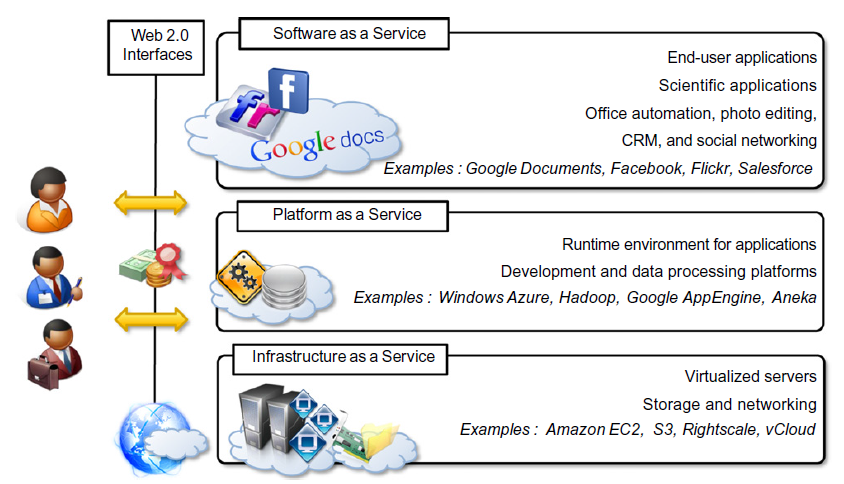
\includegraphics[scale=0.4]{service_models}}
\caption{Cloud Service Models \cite{masteringcloudcomputing}.}
\end{figure}

\textbf{Infrastructure as a Service} is the offering of virtualised resources (computation, storage, and communication) on demand\cite{vimprivatehybrid}, allowing users to provision servers on demand, running different Operating Systems and even customised software stacks. IaaS offers the advantage of control over remote resources, which is often a good fit for a company with an established IT setup looking to benefit from the cloud. It also gives the option of working with highly customised or niche software which may not be offered as a service in itself. An example of IaaS is Amazon Web Services EC2, which offers Virtual Machines with software stacks that can be customised. \cite{principlesparadigms}\\ \\
\textbf{Platform as a Service} offers a higher level of abstraction than IaaS, providing a platform which is more easily programmable. PaaS delivers scalable and elastic runtime environments on demand and host the execution of applications\cite{masteringcloudcomputing}. The cloud provider often controls scalability and manages other issues such as fault tolerance, so users can focus simply on the logic of the application utilising the cloud provider's APIs and libraries\cite{masteringcloudcomputing}. One big advantage of this approach is the lack of concern about how the cloud actually works in terms of hosting the application; instead, the user is just guaranteed a stable, scalable environment for their application to run in. Google App Engine is a great example of PaaS, allowing deployment and hosting of Web Applications\cite{googleappengine}.\\ \\
Finally, the service with the highest level of abstraction is \textbf{Software as a Service}, which as a solution provides applications and services on demand\cite{masteringcloudcomputing}, such as the common elements of desktop applications like Office Suites or photo editing. Usually these applications are accessible through a browser, and will host files and configuration data in the cloud, making for an easy access, scalable alternative to a native desktop application. Google Docs is a very popular example of SaaS, allowing editing of spreadsheets, word documents, and more, which are then stored on its sister storage service, Google Drive\cite{googledrive}.   
 
\subsection{History}
Cloud Computing has been many years in the making. Many technologies have contributed to its inception; A visualisation of these can be seen in the below figure. To understand how Cloud Computing came about, it is important to note the types of problems which were being solved, and the previous solutions that inspired this movement. 
 
\begin{figure}[ht]
\centering
\fbox{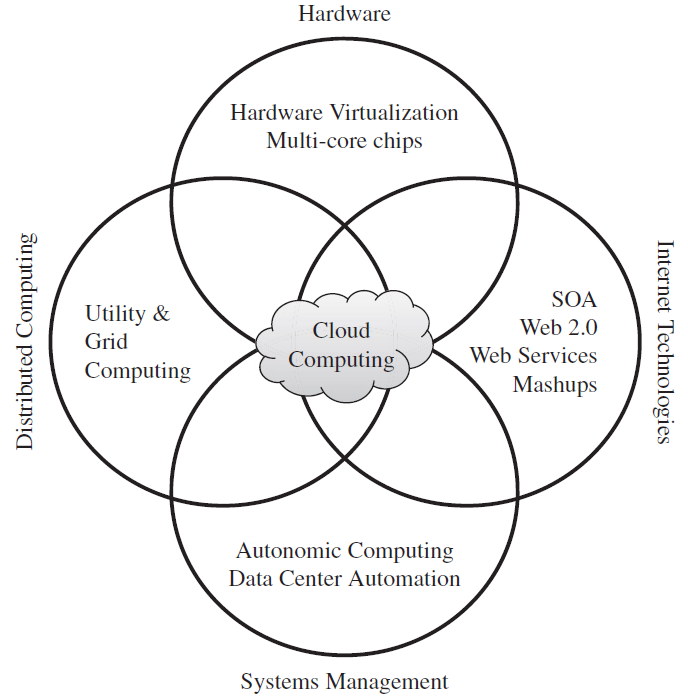
\includegraphics[scale=0.3]{roots_of_cloud_computing}}
\caption[An example figure.]{Convergence of advances leading to advent of Cloud Computing \cite{principlesparadigms}.}
\end{figure}

\textbf{Utility Computing}, i.e. the on demand delivery of infrastructure, applications, and business processes over the internet for a fee \cite{utilitybusinessmodel}, was the inspiration of a number of technologies over the years, as the idea brought great advantage to both utility providers and consumers. For providers, this meant lower operational costs, as infrastructure could be built to serve many different users, increasing efficiency and lower total cost of ownership \cite{utilityglobalgrids}. Furthermore, the economies of scale associated with building such an infrastructure allow providers such as Amazon to offer extremely low prices for their services \cite{amazonwhatiscloudcomputing}, a great benefit for consumers.  Other benefits for a consumer include the ability to adapt their usage rapidly to unpredictable needs, such as an online retailer which sees traffic spikes seasonally; more resources to handle this traffic can be acquired temporarily and released when the spike is over. Other huge advantages for company consumers are the lack of up-front infrastructure cost, and the speed and ease of deployment on the cloud \cite{amazonwhatiscloudcomputing}.    

The emergence of the \textbf{Web Service}, defined by W3C as: "\textit{A software system designed to support interoperable machine-to-machine interaction over a network}"\cite{w3cwebservice}, was a major factor in allowing the move from in-house computing power to utility-supported computing\cite{principlesparadigms}. Web Services contributed significantly to advances in software integration\cite{soapapazoglou}, gluing together applications on different platforms and hardware remotely, and allowing the free availability of information over the internet. It was this enabling of remote services that contributed to the realisation of utility computing and, eventually, the cloud. \\
Standardisation of Web Services on known technologies such as HTTP and XML made them ideal for \textbf{Service Oriented Architecture} (SOA), the purpose of which is to address the requirements of loosely coupled, distributed systems and their need for standards\cite{principlesparadigms}. \\
\textbf{Grid Computing} was one of the first major steps to realising the utility dream. It utilised the aforementioned standardised web services as a base for creating a system which aggregated distributed resources and allowed transparent access to them\cite{principlesparadigms}. Grids allowed on-demand access to computing resources over the internet. However, it was difficult to ensure Quality of Service in grids\cite{buyyamarketorientedcomputing}. This was due to a lack of performance isolation, so if resources were oversubscribed, one grid user could affect the performance given to another. Impossibility of ensuring QoS and execution time made the grid unsuitable for many applications, particularly those which were time-critical\cite{virtualworkspaces}. Virtualisation has been identified as the perfect solution for problems which have frustrated grid users. Indeed, some research projects like Globus Virtual Workspaces have added a layer to grids for virtualising computation, storage and network resources\cite{virtualworkspaces}. \\
\textbf{Hardware Virtualisation} technology, which uses hypervisor technology to split hardware resources, has contributed to the cloud through allowing data-centres to service the differing needs of consumers. The idea of virtualisation of resources for improving sharing and utilisation of computers has been established for decades\cite{surveyvmresearch}. This has now been adopted by cloud technologies such as Amazon's Elastic Compute Cloud \cite{amazonec2}. Virtualisation will be discussed in more detail later in this section. 

\subsection{Desired Characteristics \& Challenges}
In order to evaluate any Cloud technology, it is important to ascertain the characteristics of a Cloud which are more desirable, and those which present challenges to the running of a particular Cloud. In this way, it is possible to target experiments which exhibit and analyse the desirable aspects of a Cloud in a particular implementation, e.g. OpenStack, and also to perform experiments which analyse how well the implementation deals with certain well known challenges for Clouds. Some of these will require quantitative analysis, and some qualitative. 

A white paper released by Dialogic Inc.\cite{dialogiccloud} and Buyya et al.\cite{masteringcloudcomputing}\cite{principlesparadigms} identified a number of key beneficial characteristics of a Cloud. These included:

\begin{itemize}
\itemsep0em
\item Cost Savings - Reduced expenditure for increasing computing capability. Represents low barrier to entry to acquiring IT resources. 
\item Scalability / Flexibility - Growing resources and scaling back rapidly, using extra at peak times and less at off-peak. 
\item Reliability - Services using some means to support business continuity and disaster recovery. 
\item Accessibility - The ability to access a cloud in a number of ways, e.g. from a mobile as well as a standard browser. Clouds should also be available On-Demand in a Self-Service manner. 
\item Simplified application acceleration and scalability - Allowing for hosted applications to gain resources and scale up with minimal effort.
\item Energy Efficiency - Low power usage and lesser carbon footprint.
\item Efficient Resource Allocation - Lack of fragmented resources, virtual resources are allocated such that they increase performance or efficiency. 
\item Seamless creation and use of third party services - Allowing the composition of services to give flexibility of development, adding value to consumer products.
\item Elasticity - The illusion of infinite resources for a consumer. 
\item Customisation - Ability to customise resources given to consumers, by allowing root access for example.
\end{itemize}

These characteristics often represent advantages for both cloud providers and consumers, and so are usually important regardless of which service and deployment model are being used. \\ 

Cloud Computing does come with a number of challenges. Those identified by Dialogic \& Buyya et al. include:

\begin{itemize}
\itemsep0em
\item Security \& Privacy - Storing and transmitting sensitive data causes huge concern. This is especially a problem as data must be decrypted to be processed in the cloud, a 'weak point' in the chain. Often, security issues slow down deployment of cloud services. 
\item Lack of Standards - Clouds have documented interfaces; no standards are associated with these, so few clouds are interoperable. 
\item Continuous Evolution - User requirements evolve for interfaces, networking, storage, many different areas. Clouds do not remain static. 
\item Compliance Concerns - Data protection directives from the EU for example could affect cloud computing, based on what data being used. These laws can 'get in the way'. 
Technical/Practical problems - Such as with configuration, networking and sizing of complex systems. Size and scalability inherently bring such challenges. 
\item Dynamic Provisioning - Deciding on how best to provision resources, how many to provision and how long to use them for, attempting to optimise benefits from clouds.  
\end{itemize}

These are just a small number of the issues and challenges related to Clouds, and again, often cause problems regardless of cloud configurations and architectural choices. It is for this reason that products like OpenStack must address these challenges. How effectively this is achieved will be part of this evaluation.


\section{Virtualisation}
\subsection{Introduction}
Virtualisation was defined by Amit Singh \cite{virtintro} as: "\textit{a framework or methodology of dividing the resources of a computer into multiple execution environments, by applying one or more concepts
or technologies such as hardware and software partitioning, time-sharing, partial or complete machine simulation, emulation, quality of service, and many others}." \\ \\
Virtualisation provides a number of capabilities which suit the needs of Cloud providers perfectly, including hardware-independence of OS and applications, capability of provisioning a 'Virtual Machine (VM)' on any system, and single unit management of multiple OS and applications through their use as 'VM's\cite{vmwareoverview}.  \\
The main advantage of this to an IaaS cloud however, is the split created between hardware and software resources, providing flexibility to provision and allocate resources in a very dynamic manner. The below figure illustrates how this split allows a multi-purpose system to be devised from a pool of hardware using a virtual infrastructure. 

\begin{figure}[ht]
\centering
\fbox{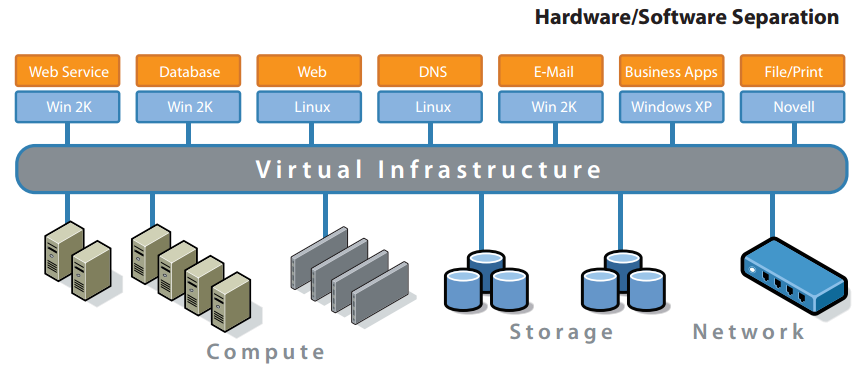
\includegraphics[scale=0.4]{hardware_separation}}
\caption{Virtual Infrastructure \cite{vmwareoverview}.}
\end{figure}

As has been previously established, Virtualisation technology is not only commonly in use in current cloud technology, but was also one of the chief driving factors contributing to the advent of Cloud Computing. Virtualisation is extremely important for products such as OpenStack due to their use as an IaaS provider. This, particularly in public cloud deployments, often means very large pools of hardware resources, such as data centres, needing the flexibility and elasticity a cloud should provide; virtualisation is key to achieving this goal. 

%\subsection{Types of Virtualisation}

\subsection{The Data Centre}
Cloud computing services are usually backed by large-scale data centers composed of thousands of computers. Such data centers are built to serve many users and host many disparate applications. For this purpose, hardware
virtualization can be considered as a perfect fit to overcome most operational
issues of data center building and maintenance\cite{principlesparadigms}. 

\begin{figure}[ht]
\centering
\fbox{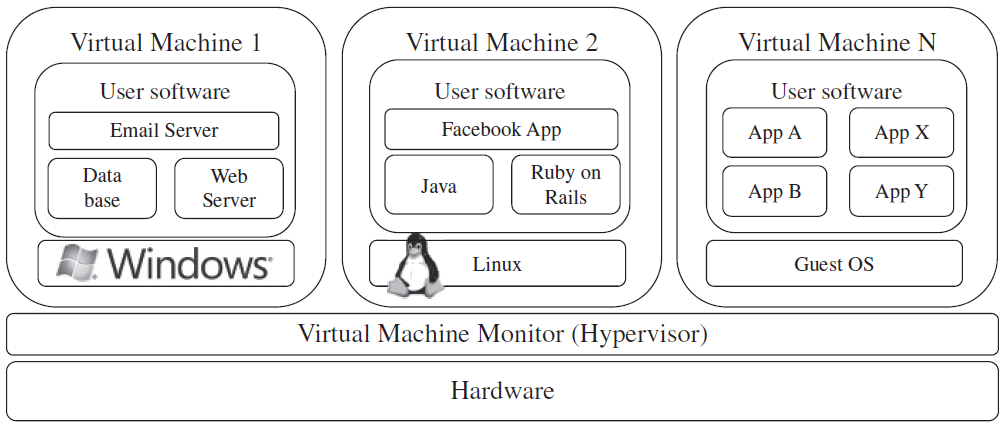
\includegraphics[scale=0.35]{vmhypervisor}}
\caption{Hardware Virtualised server hosting \cite{principlesparadigms}}
\end{figure}

This move towards the data centre has happened for a number of reasons. The first, and most obvious reason, is that use of large pools of hardware effectively utilises the capabilities of virtualisation; this power of splitting hardware in a number of ways is less effective, and often unnecessary on smaller sets of hardware.  \\
Cost Efficiency has been a huge driving factor in the trend towards the data centre and virtualisation; Virtualisation has been proven to reduce both capital expenditures (e.g. servers, storage) and operating expenses (e.g. maintenance 
 fees, management costs)\cite{agilysis}. Another enormous factor is improved server utilisation. Many data centers have servers that use anywhere from 
 5\% to 15\% of their actual capacity, with the rest going unutilized\cite{agilysis}. Due to the ability to migrate VMs and reallocate resources from certain servers to others, this figure could be greatly improved by using virtualisation, and this in turn would save money and time on power and wasted effort. \\ 
One enormous advantage of use of virtualisation, which is particularly relevant to OpenStack and this project, is the use of \textbf{Data Centre Infrastructure Management} (DCIM) solutions. Uptake of DCIM has been very high in recent years, with one analyst at Gartner stating "By 2017, DCIM tools will be significantly deployed in over 60 percent of larger data centers (over 3,000 sq ft) in North America."\cite{dcimautomation}. \\ 

DCIM is a general term for solutions aimed at improving management and automation of a data centre in terms of it's resources; those which are interesting to a cloud provider using virtualisation are \textbf{Virtual Infrastructure Managers}. These will be discussed in detail in the next part of this section. 
   
\subsection{Virtual Infrastructure Management}
Virtual Infrastructure Managers (VIMs) are software toolkits responsible for the orchestration of resources so as to rapidly and dynamically provision resources to applications\cite{vimprivatehybrid}. This type of software often resembles a traditional Operating System (OS), but instead of dealing with a single computer, it aggregates resources from multiple computers, presenting a uniform view to users and applications\cite{principlesparadigms}. Often, they are referred to as a \textbf{Cloud OS}\cite{vmwarevsphere}. \\ 
The aim of a VIM is to\cite{vimprivatehybrid}:
\begin{itemize}
\itemsep0em
\item Provide a uniform, homogeneous view of virtual resources, regardless of underlying platform. 
\item Manage the full lifecycle of a VM, including tasks like provisioning VM networks and storage. 
\item Support configurable resource allocation policies e.g. high availability, server consolidation. 
\item Adapt to the changing resource needs of an organisation. 
\end{itemize} 

\subsection{Features of VIMs}
A great number of VIMs investigated by Buyya et al.\cite{principlesparadigms} present a set of basic features related to managing VMs. These features all but define whether a tool can be used for cloud deployment. However, only a small number of those investigated exhibit features such as high availability, which allow them to be used in large-scale production clouds. These features, taken from their investigation, include:

\begin{itemize}
\itemsep0em
\item \textbf{Virtualisation Support} - Multi-tenancy in clouds requires multiple customers with disparate requirements to be serviced by the same hardware pool. Virtual resources can be resized easily with flexibility. This makes virtualisation the best option for a data centre servicing multiple tenants, as is the case with a cloud.  
\item \textbf{Self-service, On-Demand Resource Provisioning} - One of the most attractive features to a cloud. Enables users to directly obtain services from clouds, without interacting with a sysadmin. This "\textit{Eliminates the need for more time-consuming, labor-intensive, human driven procurement processes familiar to many in IT}"\cite{webspherejournal}.
\item \textbf{Multiple Backend Hypervisors} - Different virtualisation models and tools have different benefits and drawbacks. Due to this, some products offer a uniform management layer that is capable of sitting on top of many different hypervisors; in this way, a business may choose that which is right for them, or even switch without a change in how they manage their infrastructure.  
\item \textbf{Storage Virtualisation} - This means abstracting logical storage away from physical storage. By consolidating all storage in a data centre, a user can create virtual disks independent of any storage device or location. Often these are organised in a Storage Area Netwoek (SAN) and are attached to servers using protocols like Fibre Channel, iSCSI, and NFS. A storage controller provides the layer of abstraction between virtual and physical storage\cite{serverstoragevirtsingh}. Virtualisation of storage is usually more common in commercial products such as VMWare, and others just provide ways of managing storage devices. 
\item \textbf{Interface to public clouds} - Use of Cloud-bursting to extend the capacity of local in-house infrastructure is common, and if a VIM can automate or at least facilitate the 'borrowing' of capacity from a public cloud, this would be very advantageous. In this way, a VIM can support operation of a Hybrid Cloud. 
\item \textbf{Virtual Networking} - Virtual Networks allow creating an isolated network on top of physical network infrastructure independent of physical topology and locations\cite{interconnections}. A virtual LAN (VLAN) allows isolating traffic, allowing VMs to be grouped in the same networks. Most VIMs offer virtual networking capability. Some even support use of Virtual Private Networks (VPNs) for contacting local and remote VMs when using Cloud Bursting. 
\item \textbf{Dynamic Resource Allocation} - Capacity management and demand prediction are complicated in systems servicing variable and dynamic need. These problems along with awareness of energy consumption have lead to the need for dynamic resource allocation aiming at obtaining a timely match of supply and demand \cite{capacitymanagement}. Dynamically remapping VMs to physical machines at regular intervals can reduce energy consumption and better service dynamic demand. Many VIMs support features which monitor utilisation across resource pools and reallocate available resources among VMs according to application needs. 
\item \textbf{Virtual Clusters} - Some VIMs can holostically manage groups of VMs. This is useful for provisioning computing Virtual Clusters on Demand, and interconnected VMs for multi-tier Internet Applications\cite{oneclickvirtualclusters}.
\item \textbf{Reservation System} - These are systems which allow users of an infrastructure to request resources. When users request computational resources at a specific time, requests are termed advance reservations (AR). Best-effort requests are those where users request resources whenever available\cite{batchexecutionleasing} Leases on resources can be negotiated, allowing an agreement between consumer and provider. This goes a way towards allowing different users to consume the same infrastructure in a structured manner, without too much stepping on toes. 
\item \textbf{High Availability \& Data Recovery} - High Availability in VIMs aims at minimising application downtime and preventing business disruption. A few VI managers accomplish this by providing failover mechanisms, which detect both physical and virtual failures and restart VMs on healthy servers. This style of HA protects from Host, but not VM failures \cite{vmwarehighav}\cite{citrixhighav}. Sometimes, for example in critical systems, this type of failover is not enough. In this case, additional levels of fault tolerance relying on redundancy of VMs are implemented. A system will monitor when a VM or system component fails and ensures that a duplicate VM serves any application in case of failures \cite{citrixhighav}.     
\end{itemize}
Targeting experiments to exhibit these features will be a useful way to assess the capabilities of OpenStack versus its competitors. 

\subsection{Current VIM Technologies}
In order to gain some context as to the involvement of OpenStack in the Cloud Computing industry, it is important to gain some insight as to its competitors and similar products. This should also provide a good point of comparison for the evaluation of OpenStack. 
The technologies I have chosen to introduce are three of the largest and most popular current implementations. These are Eucalyptus, OpenNebula and Nimbus. A feature comparison of these three technologies can be seen in the figure below. 

\begin{figure}[ht]
\centering
\fbox{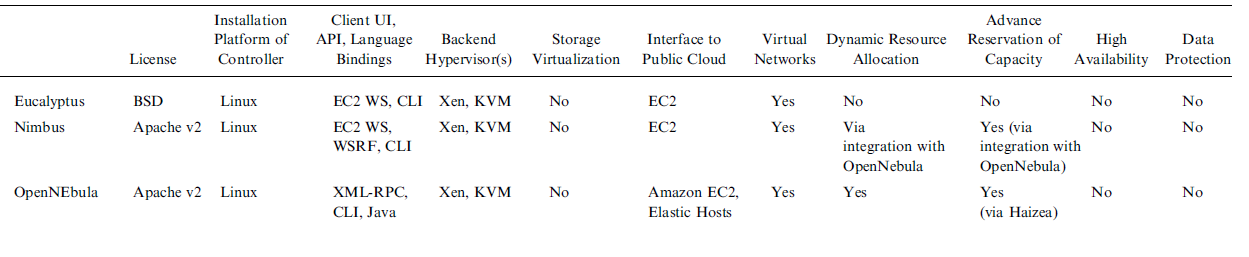
\includegraphics[scale=0.5]{VIM_comparison}}
\caption{Feature comparison of Virtual Infrastructure Managers \cite{principlesparadigms}.}
\end{figure}

\textbf{Eucalyptus}\\
Eucalpytus\cite{eucopensourcesystem} is a free, open-source tool for building Amazon Web Services (AWS) compatible private and hybrid cloud environments. It was one of the first of its kind to focus on the development of Infrastructure as a Service clouds. 
The idea behind the project was to develop an open-source implementation which would provide identical functionality and APIs to the AWS implementation, meaning that tools developed for AWS EC2, one of the most popular proprietary IaaS cloud frameworks, would also be compatible with Eucalyptus. Eucalyptus was a relatively early project, having started in 2008, but with a project called the Virtual Grid Application Development Software project, started in 2003, being one of it's main influences\cite{eucopensourcecloudsystem}.   \\ 
The project's features are split into different sections based on functionality; these, along with AWS compatibility, are Compute, Networking, Storage, Self-Service Provisioning and Cloud Management\cite{eucalyptusfeatures}. Notable features within these sections include\cite{eucalyptusfeatures}:

\begin{itemize}
\itemsep0em
\item Support for Leading Hypervisors - support for leading hypervisors such as KVM and VMware vSphere.
\item Auto Scaling - scale Eucalyptus resources up or down based on policies defined using EC2-compatible APIs and tools. 
\item CloudWatch - Provides a reliable and flexible monitoring solution for cloud resources and applications running in Eucalyptus. 
\item Elastic Load Balancing - Distributes incoming application traffic across multiple Eucalyptus instances, providing greater fault tolerance for applications.
\item Snapshot Management - snapshot and protect data stored in block storage volumes
\item Instance Management - create, manage, and delete instances.
\item Web-based Administrator Console - Performs cloud management functions such as viewing cloud resources and logs and managing virtual machine images.
\item Zero Downtime Cloud Maintenance - Leverages hypervisor live migration technologies to enable zero downtime maintenance on hardware nodes for greater application uptime.
\end{itemize}

\textbf{OpenNebula}\\
The OpenNebula project, started as a research project in 2005 by Ignacio M. Llorente and Rubén S. Montero, aims to provide efficient and scalable management of virtual machines on large-scale distributed infrastructures\cite{opennebulaaboutproject}. Due to its age, since it's first release in 2008, OpenNebula has become a mature product which solves many business needs for companies needing data centre VM management. These features allow it to be used to build public, private or hybrid IaaS clouds\cite{opennebulaabouttech}. OpenNebula is free and Open Source, under the Apache License v2, and has an active community of developers and users, with several thousand downloads per month \cite{opennebulaaboutproject}. OpenNebula appears to be a very well designed project, with objectives and design principles set in place which lead to a very clearly defined vision for the project\cite{opennebulaabouttech}.\\
Some of the key features of OpenNebula include\cite{opennebulafeatures}: 

\begin{itemize}
\itemsep0em
\item AWS EC2 and EBS APIs.
\item On-demand provision of Virtual Data Centers.
\item Automatic installation and configuration of application environments 
\item Powerful CLI that resembles typical UNIX commands applications.
\item OpenNebula Marketplace is a catalog of virtual appliances ready to run in OpenNebula environments
\item Powerful and flexible Scheduler for the definition of workload 
\item High availability architecture.
\item Cost-effective failover solution.
\end{itemize}

Interestingly, CERN, one of the largest and most advanced physics labs in the world, has recently replaced its OpenNebula environment with one using OpenStack, mainly due to the ecosystem of OpenStack being more desirable, and a number of scenario tests of OpenNebula under various conditions\cite{cernopennebula}.  

\textbf{Nimbus}\\
Nimbus is a free, open source toolkit that, once installed on a cluster, allows the provision of an IaaS cloud via Web Services. The application is aimed chiefly at the scientific community\cite{nimbusabout}. The project is based on three main goals; firstly, to enable providers of resources to build private or community IaaS clouds. Secondly, to enable users to use IaaS clouds, and thirdly, to enable developers to extend, experiment and customize IaaS\cite{nimbusabout}. This approach of considering use cases is an interesting topic of evaluation, and could be useful for this evaluation of OpenStack. \\
Notable features of Nimbus include \cite{nimbusfeatures}:
 
\begin{itemize}
\itemsep0em
\item Remote deployment and lifecycle management of VMs
\item Compatibility with Amazon's Network Protocols for EC2 and S3.
\item Easy to Use Cloud Client.
\item Per client usage tracking, per user storage quota. 
\item Configuration management at deploy time. 
\item One-click clusters - auto-configuration of entire clusters.
\item Workspace client - allows authorized clients to access all Workspace Service features. 
\item Xen and KVM plugins. 

\end{itemize}

\section{OpenStack}
\subsection{Introduction}
OpenStack is "\textit{a global collaboration of developers and cloud computing technologists producing the ubiquitous open source cloud computing platform for public and private clouds}"\cite{openstackhomepage}. The project aims to "\textit{deliver solutions for all types of clouds by being simple to implement, massively scalable, and feature rich}\cite{openstackhomepage}". The technology consists of a number of different interrelated projects all delivering various components which allow creation of cloud infrastructure. \\ 
OpenStack was founded by Rackspace Hosting and NASA, and was first publicly released in 2010. Since then, under the OpenStack foundation, the OpenStack community has grown immensely, with over 10,000 technology professionals in 133 countries having involvement in the project. Aside from the community, popularity of the product has increased greatly since its inception, and it is currently used by corporations, service providers, VARS, SMBs, researchers, and global data centers looking to deploy large-scale cloud deployments across the world. One important aspect of the product is that it is Open Source under the Apache 2.0 license, meaning that anyone can use or contribute to the project.  
Since the inception of the OpenStack foundation in 2012, more than 200 companies have joined the project, including Arista Networks, AT\&T, AMD, Brocade Communications Systems, Canonical, Cisco, Dell, EMC, Ericsson, F5 Networks, Groupe Bull, Hewlett-Packard, IBM, Inktank, Intel, NEC, NetApp, Nexenta, Rackspace Hosting, Red Hat, SUSE Linux, VMware, Oracle and Yahoo!\cite{openstackcompanies}. Many of these companies are also clients of the software. 

\subsection{Overview of Technology}
\subsubsection{Aims of the Project}
OpenStack's mission is "\textit{to enable any organization to create and offer cloud computing services running on standard hardware}" \cite{openstackhomepage}. This is a broad aim, and is the basis of the entire project. 
The long term goal of the project, taken from OpenStack's FAQ section, is "\textit{to produce the ubiquitous Open Source cloud computing platform that will meet the needs of public and private cloud providers regardless of size, by being simple to implement and massively scalable.}"\cite{openstackfaq}. Already it is clear to see that OpenStack's aims are in line with many desired cloud characteristics, such as scalability and simplicity. 
The project is targeted for use by "\textit{service providers, enterprises, government agencies and academic institutions that want to build public or private clouds. Industries range from IT \& telco to SaaS and eCommerce to finance and healthcare.}" \cite{openstackfaq}. Clearly this project is aimed at large scale, often enterprise providers, and so it will need to have high reliability and a range of capability. 
There seems to be an emphasis on the project being very open to the community. When asked 'If there are other open source cloud projects, why create a new one?' the foundation responded: "\textit{We wanted a community where people with similar philosophies about cloud architecture and open-source software can openly collaborate together. We believe in open source, open design, open development and an open community that is fully transparent? Not a cathedral, a bazaar.}"\cite{openstackfaq}
Overall, it seems that the objectives of the project are similar to those of previously created similar products, such as Eucalyptus. In this sense, OpenStack becomes a spiritual successor to these products, being the newer product, growing in popularity. 

\subsubsection{Design/Architecture of Project}
\begin{figure}[ht]
\centering
\fbox{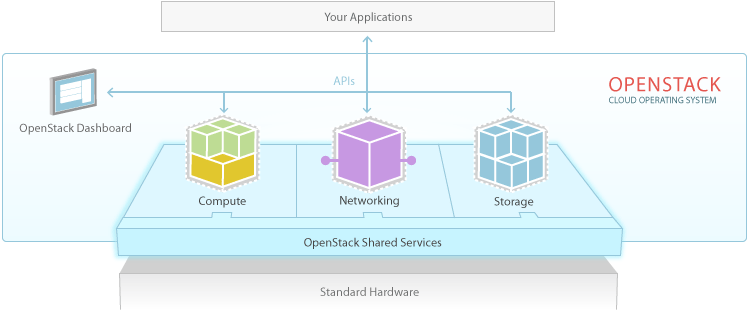
\includegraphics[scale=0.4]{openstack-software-diagram}}
\caption{Overview of OpenStack architecture \cite{openstacksoftware}.}
\end{figure}

OpenStack the project consists of a number of interrelated components, all of which work together to provide Cloud Infrastructure. These projects include\cite{openstacksoftware}:

\begin{itemize}

\item \textbf{Compute (Nova)} - Provisions and manages large networks of virtual machines.
\item \textbf{Object Storage (Swift)} - A cost effective, scale-out storage platform. 
\item \textbf{Block Storage (Cinder)} - Allows block devices to be exposed and connected to servers
\item\textbf{ Networking (Neutron)} - A Pluggable, scalable, API-driven network and IP management.
\item \textbf{Dashboard (Horizon)} - A web based Graphical User Interface for use of OpenStack.
\item \textbf{Identity Service (Keystone)} - A common authentication system across the OpenStack cloud operating system. 
\item\textbf{ Image Service (Glance)} -  Provides discovery, registration and delivery services for disk and server images. 
\item \textbf{Telemetry (Ceilometer)} -  Aggregates usage and performance data across OpenStack
\item \textbf{Orchestration (Heat)} - template-driven engine to automate the deployment of infrastructure.
\end{itemize}

\section{Current Evaluations of OpenStack}
Reading current evaluations of OpenStack gives a good idea of the types of approach and criteria used by other researchers or organisations to evaluate a product like OpenStack. Of those which were part of this literature review, a brief description of their approach and conclusions will be provided, with the hope that some inspiration can be taken for this evaluation. 

One evaluation, performed by the Engineering Task Force (ETF)\cite{etfevaluation}, gave a brief evaluation of OpenStack as part of a range of Cloud Software evaluations.
This evaluation appears to have very modest aims; simply to provide an overview of the OpenStack technology, similar to the 'Technology Overview' in this section. A brief history of the project and an overview of its components is provided in the first part of the paper. 
Another huge part of this evaluation focuses on deployment of OpenStack from the perspective of the Server and the Client; instructions of how to get a basic configuration set up are given, and a break down of some basic tasks that can be performed, such as user management, are provided. 
Finally, there is a focus on User Experience, something which is of clear importance to the ETF. This considers what the user must do to perform certain tasks involved with management and maintenance of a deployment. A short conclusion is provided, which refers to OpenStack as a "\textit{mature, well-backed software for
implementing an Infrastructure as a Service Cloud}\cite{etfevaluation}".\\
It appears that this evaluation focuses on the deployment of OpenStack and on its basic usability; it may then be a good idea to take this a step further, but with a similar approach. It has elements of both Quantitative and Qualitative evaluation, which seems a good approach. \\

A second evaluation that was covered as part of this literature review was the plan published by CERN for their own evaluation\cite{cernevaluation}. The results were not available, but the plan itself gives a very good indication of the approach taken by CERN in their evaluation, and this is clearly most important when considering how to approach another evaluation. This process appeared to be a little more developed than that of the ETF, and had a clear schedule of which tasks would be performed and evaluated. Steps included setup of hypervisors, launching of basic images, validation of dynamic shrinking and growing of resources, etc. It appears that the idea behind this particular evaluation was to analyse OpenStack by simply using it, and deliver a deployed OpenStack solution, similar to the initial aims of this evaluation. Again, a mix between qualitative research and quantitative practical work seem to be the desired approach, and one which this evaluation will likely follow. \\

From considering these two evaluations, it appears that there is a lot of room for new experimentation with OpenStack, particularly with respect to its integrated functionality and shared services. The approaches in these two, particularly CERN's approach, give a great starting point and list of tasks which have been identified as important to evaluate. These evaluations, and indeed any others that could be found, do not go into great detail, or give any comparison with other technologies, and so this is an untapped area which may provide some value, particularly for projects and organisations choosing between several solutions in future.  

\section{Plan for Evaluation of OpenStack}
\textbf{What is 'Evaluation'?}\\
When deciding to 'evaluate' OpenStack, it must be clear what is actually meant by the term 'evaluation'; the word is very vague, and evaluations can take many different forms. In order to decide, the aims \& justifications of the project must be considered:

\begin{itemize}
\itemsep0em
\item Provide knowledge of OpenStack (for the ASCETIC Project).
\item Provide some validation of OpenStack (for the ASCETIC Project).
\item Investigate the popularity of OpenStack.
\item Assess the validity of OpenStack based on its features \& capabilities.
\end{itemize}

From this, 5 main possible definitions of 'Evaluation' were drawn:

\begin{itemize}
\itemsep0em
\item Written guides of how to use OpenStack.
		\textit{This form of evaluation was used by the ETF, and was actually used for a similar purpose; as a precursor to a larger project.}
\item Functionality validation of OpenStack - i.e. validating first hand it actually does what it claims.
\textit{This was employed by CERN in their evaluation. It also was used to prepare an OpenStack deployment for another project.}
\item A review of OpenStack functionality.
\textit{Would tie in to the first two evaluations, gives an indication of how good OpenStack is based on various metrics.}
\item A comparison of OpenStack with similar competitors such as OpenNebula.
\textit{This was used by the ETF, but will be difficult in this project due to lack of resources.}
\item  A quantitative analysis of the capability of OpenStack - i.e. how well it performs certain actions.
\textit{This was not used excessively by either evaluation, but may be useful to bring new value to the domain.}
\end{itemize}

\textbf{Evaluation Considerations}\\
It is important after establishing context and analysing previous evaluations through literature review to establish some ideas concerning this evaluation of OpenStack. These can be established through a number of sources, including, but not limited to:

\begin{itemize}
\itemsep0em
\item The Aims \& Objectives of the Project - to provide some evaluation of OpenStack functionality, along with some comparison with competitors. 
\item The project deliverables - an evaluation report with designed experiments to test OpenStack, re-usable software components for use of OpenStack. 
\item The literature review - Particularly past evaluation approaches, and such useful information as desired aspects of a cloud. 
\end{itemize}

It would be extremely difficult to perform a full and advanced evaluation of all of the features of OpenStack, as it is an enormous piece of software with hundreds of use cases and features. This is where information such as the above comes in handy; it is possible to narrow the scope of this project so as to provide a fully contained and coherent evaluation, but one which does not require too much to be done than is possible in the time frame. \\

Firstly, from the recommendation of the CERN approach, the project will focus in part on use of OpenStack; experiments will be targeted at specific areas of functionality which are important, and that can be executed and demonstrated. Information from the literature review is very helpful in deciding which functionality is deemed important, as in this review, we have several guidelines on what aspects of a Cloud are important e.g. elasticity, but also those which are important to a Virtual Infrastructure Manager, e.g. multiple backend hypervisors. We even have a short overview of competitor products which should aid in qualitative feature assessment, and choice of important functionality. \\

Secondly, both of the reviewed evaluations attempt to mix qualitative and quantitative assessment, and this is something which will certainly be employed in this project; each style of assessment gives a very different view and perspective, and each can be seen as equally important, and indeed complementary when analysing software. It would of course be much easier to compare OpenStack to other implementations using qualitative assessment, as multiple deployments of different Cloud solutions is beyond the scope of this project, and so it would be difficult to obtain quantitative results to compare. \\

Finally, there are some areas in which I believe the current evaluations fall short. For a start, they do not contain any practical programmatic evaluation, and seem very focussed on systems administration. This is something which this project will attempt to include, and hopefully bring new value to this area. Furthermore, there does not appear to be much sophistication in the experiments given in previous evaluations, and this is also something which this project will attempt to tackle. Perhaps the use of programmatic automation will facilitate the ability to go into more depth when considering what functionality to assess, as it is much more difficult to manually run complex functionality from a Systems Admin's perspective. This project will aim to combine some dashboard UI experiments with automated tests, and qualitative assessment. 

\section{Conclusion}

This section has aimed to introduce \& describe the various concepts and technologies which need to be understood for this project. It has laid out concepts, referenced literature, and used this to further define the problem at hand, and how to tackle it with this project. By now, the reader should have some understanding not only of the reasons and approach of the project, but also what kind of technical work it will require, and the impact it will have on the domain. This section has aimed to provide 'context' to the project, and give it some basis in the real world. It has also aimed to further define the problem at hand, in this case an 'Evaluation' by considering previous evaluations of OpenStack, and other relevant information.  \\
In the next section, the work described in Chapters 1 \& 2 will be laid out, executed and delivered. The results of each piece of work will also be discussed. Following the next chapter, these results, and the project as a whole, will be evaluated based on a number of factors described in Chapter 4.    
